% Options for packages loaded elsewhere
\PassOptionsToPackage{unicode}{hyperref}
\PassOptionsToPackage{hyphens}{url}
%
\documentclass[
  10pt,
  letterpaper,
  DIV=11,
  numbers=noendperiod,
  twoside]{scrartcl}

\usepackage{amsmath,amssymb}
\usepackage{setspace}
\usepackage{iftex}
\ifPDFTeX
  \usepackage[T1]{fontenc}
  \usepackage[utf8]{inputenc}
  \usepackage{textcomp} % provide euro and other symbols
\else % if luatex or xetex
  \usepackage{unicode-math}
  \defaultfontfeatures{Scale=MatchLowercase}
  \defaultfontfeatures[\rmfamily]{Ligatures=TeX,Scale=1}
\fi
\usepackage{lmodern}
\ifPDFTeX\else  
    % xetex/luatex font selection
    \setmainfont[ItalicFont=EB Garamond Italic,BoldFont=EB Garamond
Bold]{EB Garamond Math}
    \setsansfont[]{Europa-Bold}
  \setmathfont[]{Garamond-Math}
\fi
% Use upquote if available, for straight quotes in verbatim environments
\IfFileExists{upquote.sty}{\usepackage{upquote}}{}
\IfFileExists{microtype.sty}{% use microtype if available
  \usepackage[]{microtype}
  \UseMicrotypeSet[protrusion]{basicmath} % disable protrusion for tt fonts
}{}
\usepackage{xcolor}
\usepackage[left=1in, right=1in, top=0.8in, bottom=0.8in,
paperheight=9.5in, paperwidth=6.5in, includemp=TRUE, marginparwidth=0in,
marginparsep=0in]{geometry}
\setlength{\emergencystretch}{3em} % prevent overfull lines
\setcounter{secnumdepth}{3}
% Make \paragraph and \subparagraph free-standing
\makeatletter
\ifx\paragraph\undefined\else
  \let\oldparagraph\paragraph
  \renewcommand{\paragraph}{
    \@ifstar
      \xxxParagraphStar
      \xxxParagraphNoStar
  }
  \newcommand{\xxxParagraphStar}[1]{\oldparagraph*{#1}\mbox{}}
  \newcommand{\xxxParagraphNoStar}[1]{\oldparagraph{#1}\mbox{}}
\fi
\ifx\subparagraph\undefined\else
  \let\oldsubparagraph\subparagraph
  \renewcommand{\subparagraph}{
    \@ifstar
      \xxxSubParagraphStar
      \xxxSubParagraphNoStar
  }
  \newcommand{\xxxSubParagraphStar}[1]{\oldsubparagraph*{#1}\mbox{}}
  \newcommand{\xxxSubParagraphNoStar}[1]{\oldsubparagraph{#1}\mbox{}}
\fi
\makeatother


\providecommand{\tightlist}{%
  \setlength{\itemsep}{0pt}\setlength{\parskip}{0pt}}\usepackage{longtable,booktabs,array}
\usepackage{calc} % for calculating minipage widths
% Correct order of tables after \paragraph or \subparagraph
\usepackage{etoolbox}
\makeatletter
\patchcmd\longtable{\par}{\if@noskipsec\mbox{}\fi\par}{}{}
\makeatother
% Allow footnotes in longtable head/foot
\IfFileExists{footnotehyper.sty}{\usepackage{footnotehyper}}{\usepackage{footnote}}
\makesavenoteenv{longtable}
\usepackage{graphicx}
\makeatletter
\newsavebox\pandoc@box
\newcommand*\pandocbounded[1]{% scales image to fit in text height/width
  \sbox\pandoc@box{#1}%
  \Gscale@div\@tempa{\textheight}{\dimexpr\ht\pandoc@box+\dp\pandoc@box\relax}%
  \Gscale@div\@tempb{\linewidth}{\wd\pandoc@box}%
  \ifdim\@tempb\p@<\@tempa\p@\let\@tempa\@tempb\fi% select the smaller of both
  \ifdim\@tempa\p@<\p@\scalebox{\@tempa}{\usebox\pandoc@box}%
  \else\usebox{\pandoc@box}%
  \fi%
}
% Set default figure placement to htbp
\def\fps@figure{htbp}
\makeatother
% definitions for citeproc citations
\NewDocumentCommand\citeproctext{}{}
\NewDocumentCommand\citeproc{mm}{%
  \begingroup\def\citeproctext{#2}\cite{#1}\endgroup}
\makeatletter
 % allow citations to break across lines
 \let\@cite@ofmt\@firstofone
 % avoid brackets around text for \cite:
 \def\@biblabel#1{}
 \def\@cite#1#2{{#1\if@tempswa , #2\fi}}
\makeatother
\newlength{\cslhangindent}
\setlength{\cslhangindent}{1.5em}
\newlength{\csllabelwidth}
\setlength{\csllabelwidth}{3em}
\newenvironment{CSLReferences}[2] % #1 hanging-indent, #2 entry-spacing
 {\begin{list}{}{%
  \setlength{\itemindent}{0pt}
  \setlength{\leftmargin}{0pt}
  \setlength{\parsep}{0pt}
  % turn on hanging indent if param 1 is 1
  \ifodd #1
   \setlength{\leftmargin}{\cslhangindent}
   \setlength{\itemindent}{-1\cslhangindent}
  \fi
  % set entry spacing
  \setlength{\itemsep}{#2\baselineskip}}}
 {\end{list}}
\usepackage{calc}
\newcommand{\CSLBlock}[1]{\hfill\break\parbox[t]{\linewidth}{\strut\ignorespaces#1\strut}}
\newcommand{\CSLLeftMargin}[1]{\parbox[t]{\csllabelwidth}{\strut#1\strut}}
\newcommand{\CSLRightInline}[1]{\parbox[t]{\linewidth - \csllabelwidth}{\strut#1\strut}}
\newcommand{\CSLIndent}[1]{\hspace{\cslhangindent}#1}

\setlength\heavyrulewidth{0ex}
\setlength\lightrulewidth{0ex}
\usepackage[automark]{scrlayer-scrpage}
\clearpairofpagestyles
\cehead{
  Brian Weatherson
  }
\cohead{
  Changes in Citation Patterns
  }
\ohead{\bfseries \pagemark}
\cfoot{}
\makeatletter
\newcommand*\NoIndentAfterEnv[1]{%
  \AfterEndEnvironment{#1}{\par\@afterindentfalse\@afterheading}}
\makeatother
\NoIndentAfterEnv{itemize}
\NoIndentAfterEnv{enumerate}
\NoIndentAfterEnv{description}
\NoIndentAfterEnv{quote}
\NoIndentAfterEnv{equation}
\NoIndentAfterEnv{longtable}
\NoIndentAfterEnv{abstract}
\renewenvironment{abstract}
 {\vspace{-1.25cm}
 \quotation\small\noindent\rule{\linewidth}{.5pt}\par\smallskip
 \noindent }
 {\par\noindent\rule{\linewidth}{.5pt}\endquotation}
\KOMAoption{captions}{tableheading}
\makeatletter
\@ifpackageloaded{caption}{}{\usepackage{caption}}
\AtBeginDocument{%
\ifdefined\contentsname
  \renewcommand*\contentsname{Table of contents}
\else
  \newcommand\contentsname{Table of contents}
\fi
\ifdefined\listfigurename
  \renewcommand*\listfigurename{List of Figures}
\else
  \newcommand\listfigurename{List of Figures}
\fi
\ifdefined\listtablename
  \renewcommand*\listtablename{List of Tables}
\else
  \newcommand\listtablename{List of Tables}
\fi
\ifdefined\figurename
  \renewcommand*\figurename{Figure}
\else
  \newcommand\figurename{Figure}
\fi
\ifdefined\tablename
  \renewcommand*\tablename{Table}
\else
  \newcommand\tablename{Table}
\fi
}
\@ifpackageloaded{float}{}{\usepackage{float}}
\floatstyle{ruled}
\@ifundefined{c@chapter}{\newfloat{codelisting}{h}{lop}}{\newfloat{codelisting}{h}{lop}[chapter]}
\floatname{codelisting}{Listing}
\newcommand*\listoflistings{\listof{codelisting}{List of Listings}}
\makeatother
\makeatletter
\makeatother
\makeatletter
\@ifpackageloaded{caption}{}{\usepackage{caption}}
\@ifpackageloaded{subcaption}{}{\usepackage{subcaption}}
\makeatother

\usepackage{bookmark}

\IfFileExists{xurl.sty}{\usepackage{xurl}}{} % add URL line breaks if available
\urlstyle{same} % disable monospaced font for URLs
\hypersetup{
  pdftitle={Changes in Citation Patterns},
  pdfauthor={Brian Weatherson},
  hidelinks,
  pdfcreator={LaTeX via pandoc}}


\title{Changes in Citation Patterns}
\author{Brian Weatherson}
\date{2024}

\begin{document}
\maketitle
\begin{abstract}
By looking at changes in citation patterns, we can tell something about
the way in which academic philosophy has changed over the last few
decades. One thing that stands out is the reduction in armchair
approaches to non-fundamental questions. Another is that topics no
longer disappear from philosophy. Since around 2002, every topic that
has reached a certain level of prominence in the literature has retained
its prominence. This is notably not the case before the late 1990s.
\end{abstract}


\setstretch{1.1}
By looking at changes in citation patterns, we can tell something about
the way in which academic philosophy has changed over the last few
decades. One thing that stands out is the reduction in armchair
approaches to non-fundamental questions. Another is that topics no
longer disappear from philosophy. Since around 2002, every topic that
has reached a certain level of prominence in the literature has retained
its prominence. This is notably not the case before the late 1990s.

\section{Introduction}\label{sec-introduction}

This paper is about citations of philosophy journal articles in
philosophy journal articles. The data comes from Web of Science. I'm
focussing on citations between philosophy journals for two reasons. One
is that the data is much cleaner. Citations to books, chapters, theses,
and other sources, requires a lot of work to be even approximately
correct, while citations of journals in journals are reasonably
reliable. (This is especially true for journals that use end of article
bibliographies; there the reliability is very high.) The second is that
the data is complete. It's very hard to get a complete list of all the
philosophy books published in a year, or even conceptually to think
about what that would mean. It's much easier to find some journals, and
get a complete list of their articles.

I'm focusing on journals published since 1965. So the citations are of
articles published since 1965, in articles published since 1965. That
means that at the start there are very few citations, since most
citations are to things a few years earlier.

One problem with using Web of Science is that it is very slow to update.
I'm using the XML files that are provided to subscribing institutions.
The most recent such files that are provided only go through mid-2022.
Much of the focus here is on citations since 2020. Crucially, this does
not mean 2020-2024; it just means 2020-to-mid-2022. This still turns out
to be a lot of citations.

Web of Science is also slow to add journals to its index. As
Table~\ref{tbl-list-of-journals} shows, several journals are only added
to the index well after 1965, or (in the case of some recently founded
journals) well after their founding. The biggest impact this has on this
paper is that we don't have the citation data for \emph{Analysis} before
1975, and that probably affects some of the results.

I'm also focusing on one hundred journals. I downloaded the citation
data for every journal in the categories Philosophy, and History and
Philosophy of Science, and picked out the hundred journals with the most
articles, which seemed to be primarily English language, analytic, and
philosophy as opposed to history of science journals. The journals that
I picked are listed in Table~\ref{tbl-list-of-journals}.

\begin{longtable}[]{@{}
  >{\raggedright\arraybackslash}p{(\linewidth - 6\tabcolsep) * \real{0.5747}}
  >{\raggedleft\arraybackslash}p{(\linewidth - 6\tabcolsep) * \real{0.1034}}
  >{\raggedleft\arraybackslash}p{(\linewidth - 6\tabcolsep) * \real{0.1264}}
  >{\raggedleft\arraybackslash}p{(\linewidth - 6\tabcolsep) * \real{0.1954}}@{}}

\caption{\label{tbl-list-of-journals}The journals included in this
study.}

\tabularnewline

\toprule\noalign{}
\begin{minipage}[b]{\linewidth}\raggedright
Journal
\end{minipage} & \begin{minipage}[b]{\linewidth}\raggedleft
Articles
\end{minipage} & \begin{minipage}[b]{\linewidth}\raggedleft
First Year
\end{minipage} & \begin{minipage}[b]{\linewidth}\raggedleft
Most Recent Year
\end{minipage} \\
\midrule\noalign{}
\endhead
\bottomrule\noalign{}
\endlastfoot
Acta Philosophica & 211 & 2009 & 2022 \\
American Philosophical Quarterly & 1755 & 1964 & 2021 \\
Analysis & 2615 & 1975 & 2022 \\
Analytic Philosophy & 169 & 2016 & 2022 \\
Archiv Fur Geschichte Der Philosophie & 676 & 1975 & 2022 \\
Australasian Journal Of Philosophy & 1683 & 1975 & 2022 \\
Biology \& Philosophy & 1117 & 1988 & 2022 \\
British Journal For The History Of Philosophy & 760 & 2007 & 2022 \\
British Journal For The Philosophy Of Science & 1499 & 1956 & 2022 \\
British Journal Of Aesthetics & 1369 & 1975 & 2022 \\
Bulletin Of Symbolic Logic & 81 & 2003 & 2022 \\
Canadian Journal Of Philosophy & 1497 & 1975 & 2022 \\
Croatian Journal Of Philosophy & 329 & 2007 & 2022 \\
Dialogue & 1464 & 1975 & 2022 \\
Economics And Philosophy & 116 & 2003 & 2022 \\
Episteme & 551 & 2005 & 2022 \\
Ergo & 213 & 2016 & 2021 \\
Erkenntnis & 1744 & 2000 & 2022 \\
Ethical Theory And Moral Practice & 854 & 2008 & 2022 \\
Ethics & 1564 & 1956 & 2022 \\
European Journal For Philosophy Of Science & 449 & 2011 & 2022 \\
European Journal Of Philosophy & 914 & 1998 & 2022 \\
Heythrop Journal & 792 & 1975 & 2014 \\
History And Philosophy Of Logic & 475 & 1992 & 2022 \\
Hume Studies & 111 & 2010 & 2022 \\
Hypatia & 607 & 2009 & 2022 \\
Inquiry & 1743 & 1966 & 2022 \\
International Journal For Philosophy Of Religion & 1098 & 1975 & 2022 \\
International Philosophical Quarterly & 1543 & 1961 & 2022 \\
Journal Of Aesthetics And Art Criticism & 1473 & 1975 & 2022 \\
Journal Of Applied Philosophy & 607 & 2006 & 2022 \\
Journal Of Chinese Philosophy & 1234 & 1973 & 2022 \\
Journal Of Consciousness Studies & 1356 & 2000 & 2022 \\
Journal Of Indian Philosophy & 1034 & 1975 & 2022 \\
Journal Of Medical Ethics & 270 & 1975 & 2022 \\
Journal Of Moral Philosophy & 347 & 2005 & 2022 \\
Journal Of Philosophical Logic & 1411 & 1972 & 2022 \\
Journal Of Philosophical Research & 508 & 2005 & 2022 \\
Journal Of Philosophy & 2474 & 1956 & 2022 \\
Journal Of Political Philosophy & 282 & 2003 & 2022 \\
Journal Of Social Philosophy & 481 & 2008 & 2022 \\
Journal Of Symbolic Logic & 192 & 1968 & 2022 \\
Journal Of The American Philosophical Association & 306 & 2015 & 2022 \\
Journal Of The History Of Ideas & 2101 & 1956 & 2022 \\
Journal Of The History Of Philosophy & 1083 & 1975 & 2022 \\
Journal Of The Philosophy Of History & 239 & 2010 & 2022 \\
Journal Of Value Inquiry & 1358 & 1980 & 2022 \\
Kant-Studien & 1068 & 1975 & 2022 \\
Kantian Review & 293 & 2010 & 2022 \\
Kennedy Institute Of Ethics Journal & 551 & 1995 & 2022 \\
Law And Philosophy & 208 & 2003 & 2022 \\
Logique Et Analyse & 339 & 2007 & 2021 \\
Metaphilosophy & 1470 & 1975 & 2022 \\
Midwest Studies In Philosophy & 107 & 1984 & 1988 \\
Mind & 1906 & 1956 & 2022 \\
Mind \& Language & 155 & 2003 & 2022 \\
Minds And Machines & 192 & 2003 & 2022 \\
Monist & 1911 & 1962 & 2022 \\
Notre Dame Journal Of Formal Logic & 424 & 2009 & 2022 \\
Noûs & 1443 & 1975 & 2022 \\
Pacific Philosophical Quarterly & 1190 & 1980 & 2022 \\
Philosophers' Imprint & 353 & 2010 & 2022 \\
Philosophia & 2050 & 1975 & 2022 \\
Philosophia Mathematica & 221 & 2008 & 2022 \\
Philosophical Explorations & 353 & 2008 & 2022 \\
Philosophical Forum & 802 & 1971 & 2022 \\
Philosophical Investigations & 676 & 1983 & 2022 \\
Philosophical Papers & 225 & 2009 & 2022 \\
Philosophical Perspectives & 275 & 2007 & 2022 \\
Philosophical Psychology & 291 & 2003 & 2022 \\
Philosophical Quarterly & 1341 & 1975 & 2022 \\
Philosophical Review & 988 & 1956 & 2022 \\
Philosophical Studies & 5210 & 1956 & 2022 \\
Philosophical Topics & 106 & 1981 & 1986 \\
Philosophy & 1951 & 1956 & 2022 \\
Philosophy \& Public Affairs & 698 & 1971 & 2022 \\
Philosophy And Phenomenological Research & 3149 & 1956 & 2022 \\
Philosophy And Rhetoric & 886 & 1975 & 2022 \\
Philosophy Compass & 540 & 2015 & 2022 \\
Philosophy East \& West & 1488 & 1966 & 2022 \\
Philosophy Of Science & 3020 & 1956 & 2022 \\
Philosophy Of The Social Sciences & 914 & 1975 & 2022 \\
Phronesis & 743 & 1975 & 2022 \\
Politics Philosophy \& Economics & 195 & 2008 & 2022 \\
Ratio & 1040 & 1974 & 2022 \\
Review Of Metaphysics & 1560 & 1956 & 2022 \\
Review Of Symbolic Logic & 535 & 2008 & 2022 \\
Russell & 379 & 1975 & 2022 \\
Social Philosophy \& Policy & 893 & 1983 & 2021 \\
South African Journal Of Philosophy & 726 & 1987 & 2022 \\
Southern Journal Of Philosophy & 1899 & 1976 & 2022 \\
Southwestern Journal Of Philosophy & 422 & 1970 & 1980 \\
Studia Logica & 666 & 2010 & 2022 \\
Studies In History And Philosophy Of Science & 1660 & 1974 & 2022 \\
Synthese & 6978 & 1966 & 2022 \\
Theoria & 395 & 2007 & 2022 \\
Thought & 188 & 2016 & 2021 \\
Topoi & 1113 & 1982 & 2022 \\
Transactions Of The Charles S Peirce Society & 1132 & 1975 & 2022 \\
Utilitas & 360 & 2009 & 2022 \\

\end{longtable}

Of course the first year isn't the first year the journal started
publishing; it's when Web of Science started indexing them. And the last
year isn't when they ceased publishing; it's the most recent year
indexed. Web of Science is very slow at adding journals, and at adding
volumes. But it is, as far as I've found, pretty accurate within what it
adds.

One big exception to this is that it's never really understood how to
handle the `supplements' to \emph{Noûs}, i.e., \emph{Philosophical
Perspectives} and \emph{Philosophical Issues}. Some of these are
recorded as being their own thing, some of them are recorded as special
issues of \emph{Noûs}. In the latter case, the citations often only
start being tracked several years after publication, and the
bibliographic information is spotty. I've manually removed the ones that
were listed as being published in \emph{Noûs} but actually in one of the
supplements, because the data didn't seem sufficiently reliable. The
major cost of this is that Kit Fine's paper ``Essence and Modality''
isn't part of the study; this is something that I might need to correct.

I've also manually added citations to articles published in
\emph{Journal of Philosophy} between 1971 and 1974. I don't have good
data for what was cited in those articles. I don't know why Web of
Science indexes the Journal before and after that period, but it's an
important gap. Several of the most important articles of the journals
era are published in the Journal in those years, so I felt it was
important to include them. I hope that the manual adding I did led to
values on the same scale as what I got from everything else, but this is
a possible source of noise in the data.

Because Web of Science keeps adding journals, and journals keep getting
larger, the number of articles in this study keeps going up. The only
downward pressure comes from the fact that some journals haven't been
indexed for 2022 or even, in some cases, 2021.
Figure~\ref{fig-number-of-articles-by-year} shows how many articles each
year are in the study.

\begin{figure}

\centering{

\pandocbounded{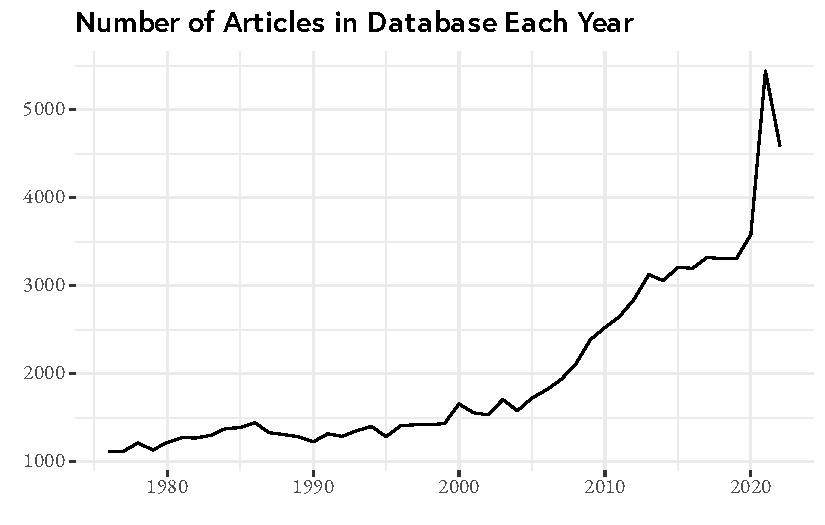
\includegraphics[keepaspectratio]{changes_files/figure-pdf/fig-number-of-articles-by-year-1.pdf}}

}

\caption{\label{fig-number-of-articles-by-year}Number of articles in the
study each year}

\end{figure}%

On top of that, citation practices have changed and people now cite much
more widely than they used to. So the number of citations recorded each
year (to articles since 1965 indexed in these hundred journals), has
risen rather dramatically, as shown in
Figure~\ref{fig-number-of-citations-by-year}.

\begin{figure}

\centering{

\pandocbounded{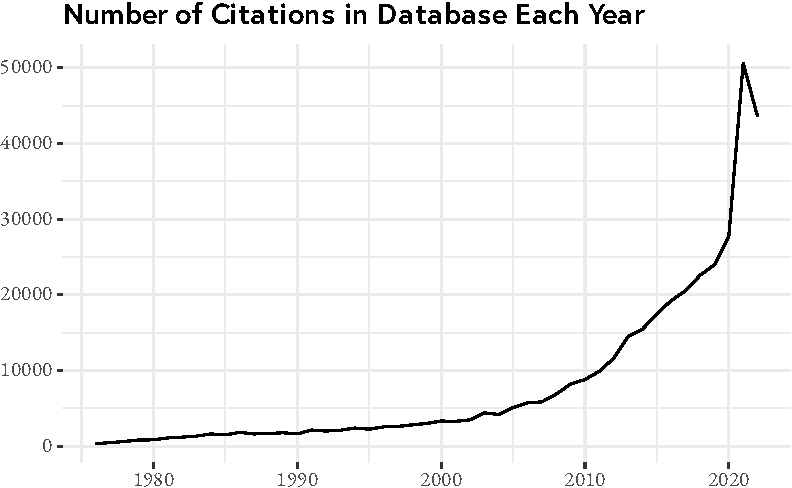
\includegraphics[keepaspectratio]{changes_files/figure-pdf/fig-number-of-citations-by-year-1.pdf}}

}

\caption{\label{fig-number-of-citations-by-year}Number of citations to
articles in the study each year}

\end{figure}%

On the other hand, since the overwhelming majority of citations are to
articles published earlier than the citing article, a larger number of
citations in total might be consistent with fewer citations per article
available to be cited. If we somewhat arbitrarily set the universe of
available to be cited papers as the set of papers with the same
publication date as the citing article or earlier,
Figure~\ref{fig-average-of-citations-by-year} shows how often the
average paper was cited each year (in these 100 journals).

\begin{figure}

\centering{

\pandocbounded{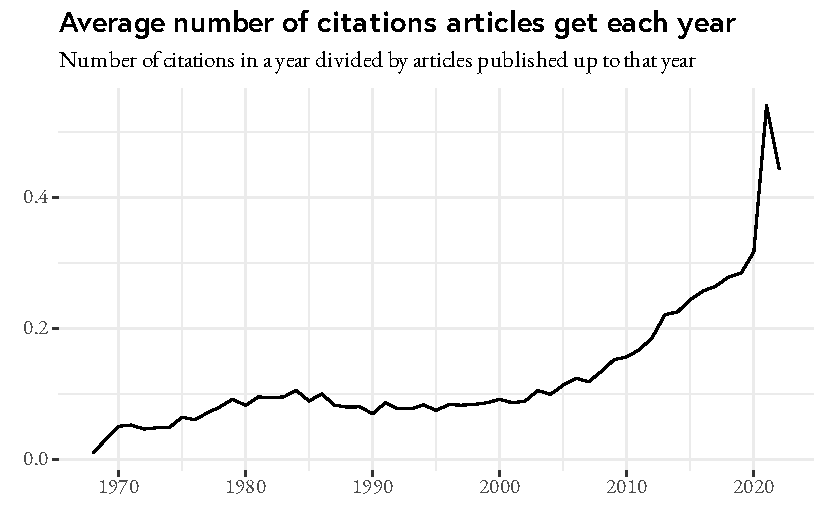
\includegraphics[keepaspectratio]{changes_files/figure-pdf/fig-average-of-citations-by-year-1.pdf}}

}

\caption{\label{fig-average-of-citations-by-year}Average number of
citations per available article in each year}

\end{figure}%

Between about 1978 and 2004, the different forces are roughly balanced.
There are more papers, and each paper cites more often, but there are
more papers available to be cited, and the mean stays at about 0.1. But
then the forces pushing this number up take over.

\section{Recent Citations}\label{sec-recent-citations}

The focus here is going to be on articles whose recent citation patterns
are markedly different to their citation pattern since 2020. To
understand these, it helps to have a sense of what the citations since
2020 are like.

The first thing to know about the 2020s is that the number of outbound
citations per article shot up, starting in 2021. This is shown in
\textbf{?@fig-outbound-citation-rate}.

\begin{figure}

\centering{

\pandocbounded{\includegraphics[keepaspectratio]{changes_files/figure-pdf/fig-average-of-outbound-citations-by-year-1.pdf}}

}

\caption{\label{fig-average-of-outbound-citations-by-year}Average number
of outbound citations in each year}

\end{figure}%

Remember these are outbound citations to philosophy journal articles
published since 1965. At the left hand edge of
Figure~\ref{fig-average-of-outbound-citations-by-year}, the `since 1965'
constraint probably makes a big difference to the graph. It shouldn't
really make a difference towards the right of the graph, and yet the
line keeps going up.

Between the number of articles published since 2020, and the high rate
of outbound citations in those articles, there are a lot of citations
since 2020. The whole study, from 1965 to 2022, includes 379532
citations. The part since 2020 alone includes 121043 of those citations.

The study contains 99252 papers. So the average paper was cited about
1.2 times since 2020. Citations are not distributed at all evenly.
Table~\ref{tbl-count-of-recent-citations} shows how many articles have
at least \emph{n} citations since 2020 for various values of \emph{n}.

\begin{longtable}[]{@{}rr@{}}

\caption{\label{tbl-count-of-recent-citations}Frequency of articles with
at least n citations, for various values of n}

\tabularnewline

\toprule\noalign{}
n & Number of articles \\
\midrule\noalign{}
\endhead
\bottomrule\noalign{}
\endlastfoot
1 & 32938 \\
2 & 18818 \\
3 & 12417 \\
4 & 9007 \\
5 & 6879 \\
6 & 5389 \\
7 & 4288 \\
8 & 3519 \\
9 & 2903 \\
10 & 2448 \\
15 & 1214 \\
20 & 697 \\
25 & 448 \\
30 & 315 \\
35 & 221 \\
40 & 159 \\
45 & 112 \\
50 & 88 \\

\end{longtable}

Just over 1\% of articles have at least fifteen citations since 2020.
Just under 0.1\% have at least fifty citations. I'll sometimes talk
below about articles that were once the center of attention having
`only' five citations since 2020. It's worth remembering that this still
means they are in the top 7\% or so for citations over that time. Most
things don't get cited, at least in other philosophy journals in this
time period.

The very top of the citation list, since 2020, is shown in
Table~\ref{tbl-recent-high-cite}.


\begin{longtable}[]{@{}
  >{\raggedleft\arraybackslash}p{(\linewidth - 2\tabcolsep) * \real{0.0833}}
  >{\raggedright\arraybackslash}p{(\linewidth - 2\tabcolsep) * \real{0.9167}}@{}}

\caption{\label{tbl-recent-high-cite}Twenty most cited articles since
2020}

\tabularnewline

\toprule\noalign{}
\begin{minipage}[b]{\linewidth}\raggedleft
Late Cites
\end{minipage} & \begin{minipage}[b]{\linewidth}\raggedright
Article
\end{minipage} \\
\midrule\noalign{}
\endhead
\bottomrule\noalign{}
\endlastfoot
246 & David Lewis
(\citeproc{ref-WOSA1983RR51600001}{1983})
``New Work for a Theory of Universals'' \\
156 & S Haslanger
(\citeproc{ref-WOS000085841900002}{2000})
``Gender and Race: (What) Are They? (What) Do We Want Them To Be?'' \\
127 & P Machamer, L Darden, et al
(\citeproc{ref-WOS000087305900001}{2000})
``Thinking About Mechanisms'' \\
112 & A Clark and D Chalmers
(\citeproc{ref-WOS000073222300002}{1998})
``The Extended Mind'' \\
111 & Jonathan Schaffer
(\citeproc{ref-WOS000368189400004}{2016})
``Grounding in the Image of Causation'' \\
108 & T Nagel
(\citeproc{ref-WOSA1974U469700001}{1974})
``What is It Like To Be a Bat'' \\
107 & David Lewis
(\citeproc{ref-WOSA1996VY21200001}{1996})
``Elusive Knowledge'' \\
105 & Jessica M. Wilson
(\citeproc{ref-WOS000344393500001}{2014})
``No Work for a Theory of Grounding'' \\
100 & J Pryor
(\citeproc{ref-WOS000165361800002}{2000})
``The Skeptic and the Dogmatist'' \\
100 & John Hawthorne and Jason Stanley
(\citeproc{ref-WOS000262624000001}{2008})
``Knowledge and Action'' \\
99 & David Plunkett and Tim Sundell
(\citeproc{ref-WOS000332023600001}{2013})
``Disagreement and the Semantics of Normative and Evaluative Terms'' \\
97 & Adam Elga
(\citeproc{ref-WOS000249103800005}{2007})
``Reflection and Disagreement'' \\
96 & JM Joyce
(\citeproc{ref-WOS000077956100002}{1998})
``A Nonpragmatic Vindication of Probabilism'' \\
96 & S Kripke
(\citeproc{ref-WOSA1975BF60000005}{1975})
``Outline of a Theory of Truth'' \\
95 & HG Frankfurt
(\citeproc{ref-WOSA1969Y444700002}{1969})
``Alternate Possibilities and Moral Responsibility'' \\
95 & P Singer
(\citeproc{ref-WOSA1972Z066400001}{1972})
``Famine, Affluence, and Morality'' \\
94 & David Christensen
(\citeproc{ref-WOS000207419300002}{2007})
``Epistemology of Disagreement: The Good News'' \\
94 & David Lewis
(\citeproc{ref-WOSA1979HJ57600007}{1979c})
``Scorekeeping in a Language Game'' \\
91 & ES Anderson
(\citeproc{ref-WOS000078432400003}{1999})
``What is the Point of Equality?'' \\
90 & Kristie Dotson
(\citeproc{ref-WOS000289948200002}{2011})
``Tracking Epistemic Violence, Tracking Practices of Silencing'' \\

\end{longtable}

The most recent article in that list is from 2016. That might lead you
to think that philosophy citations are typically to rather old articles.
This isn't true. Figure~\ref{fig-recent-cite-rate} shows how often, on
average, papers with different publication years are cited since 2020.

\begin{figure}

\centering{

\pandocbounded{\includegraphics[keepaspectratio]{changes_files/figure-pdf/fig-recent-cite-rate-1.pdf}}

}

\caption{\label{fig-recent-cite-rate}Average number of cites since 2020
by year of original publication}

\end{figure}%

The peak is actually in 2018. Recently published articles are, on
average, cited more than articles from longer ago. It's just that the
citations are more widely spread out.
Table~\ref{tbl-recent-from-last-five} shows which articles since 2016
have the most citations since 2020.


\begin{longtable}[]{@{}
  >{\raggedleft\arraybackslash}p{(\linewidth - 2\tabcolsep) * \real{0.0764}}
  >{\raggedright\arraybackslash}p{(\linewidth - 2\tabcolsep) * \real{0.9236}}@{}}

\caption{\label{tbl-recent-from-last-five}Twenty most cited articles
since 2020, first published since 2016.}

\tabularnewline

\toprule\noalign{}
\begin{minipage}[b]{\linewidth}\raggedleft
Late Cites
\end{minipage} & \begin{minipage}[b]{\linewidth}\raggedright
Article
\end{minipage} \\
\midrule\noalign{}
\endhead
\bottomrule\noalign{}
\endlastfoot
111 & Jonathan Schaffer
(\citeproc{ref-WOS000368189400004}{2016})
``Grounding in the Image of Causation'' \\
75 & Alexander Skiles
(\citeproc{ref-WOS000360509700002}{2015})
``Against Grounding Necessitarianism'' \\
67 & Cian Dorr
(\citeproc{ref-WOS000397575900003}{2016})
``To Be F is To Be G'' \\
66 & Alison Hills
(\citeproc{ref-WOS000387458900001}{2016})
``Understanding Why'' \\
58 & Jane Friedman
(\citeproc{ref-WOS000400022600006}{2017})
``Why Suspend Judging?'' \\
56 & Alastair Wilson
(\citeproc{ref-WOS000449886300001}{2018})
``Metaphysical Causation'' \\
51 & Jane Friedman
(\citeproc{ref-WOS000465095900003}{2019})
``Inquiry and Belief'' \\
49 & David Plunkett
(\citeproc{ref-WOS000366669500008}{2015})
``Which Concepts Should We Use?: Metalinguistic Negotiations and the
Methodology of Philosophy'' \\
49 & Jonathan Schaffer
(\citeproc{ref-WOS000404667500001}{2017})
``The Ground Between the Gaps'' \\
47 & Miranda Fricker
(\citeproc{ref-WOS000368807300008}{2016})
``What's the Point of Blame? A Paradigm Based Explanation'' \\
47 & Conor Mchugh and Jonathan Way
(\citeproc{ref-WOS000373095100002}{2016})
``Fittingness First'' \\
45 & Georg Brun
(\citeproc{ref-WOS000388169500004}{2016})
``Explication as a Method of Conceptual Re-Engineering'' \\
45 & Rima Basu
(\citeproc{ref-WOS000477039200013}{2019})
``The Wrongs of Racist Beliefs'' \\
44 & John Hawthorne, Daniel Rothschild, et al
(\citeproc{ref-WOS000373229500014}{2016})
``Belief is Weak'' \\
43 & Michael J. Raven
(\citeproc{ref-WOS000359831800003}{2015})
``Ground'' \\
43 & David J. Chalmers
(\citeproc{ref-WOS000445442600001}{2018})
``The Meta-Problem of Consciousness'' \\
42 & Alex Worsnip
(\citeproc{ref-WOS000419946900001}{2018})
``The Conflict of Evidence and Coherence'' \\
42 & C. Thi Nguyen
(\citeproc{ref-WOS000539283800001}{2020})
``Echo Chambers and Epistemic Bubbles'' \\
41 & Katharine Jenkins
(\citeproc{ref-WOS000366750800006}{2016})
``Amelioration and Inclusion: Gender Identity and the Concept of
Woman'' \\
41 & Shamik Dasgupta
(\citeproc{ref-WOS000374968600007}{2016})
``Metaphysical Rationalism'' \\

\end{longtable}

The list of authors there is a little less white, and a little less
male, than most of the lists we'll see below. As we'll see, that's not
saying much.

Many of the articles that were recently widely cited have been cited a
lot almost as soon as they were published. But not all of them were.
Table~\ref{tbl-very-late-bloomers} lists the articles with the most
cites since 2020 that were, in a sense I'll get to below, not widely
cited when they were first published.


\begin{longtable}[]{@{}
  >{\raggedleft\arraybackslash}p{(\linewidth - 2\tabcolsep) * \real{0.0833}}
  >{\raggedright\arraybackslash}p{(\linewidth - 2\tabcolsep) * \real{0.9167}}@{}}

\caption{\label{tbl-very-late-bloomers}Twenty most cited articles since
2020 that were not (as) widely cited when they were published.}

\tabularnewline

\toprule\noalign{}
\begin{minipage}[b]{\linewidth}\raggedleft
Citations
\end{minipage} & \begin{minipage}[b]{\linewidth}\raggedright
Article
\end{minipage} \\
\midrule\noalign{}
\endhead
\bottomrule\noalign{}
\endlastfoot
156 & S Haslanger
(\citeproc{ref-WOS000085841900002}{2000})
``Gender and Race: (What) Are They? (What) Do We Want Them To Be?'' \\
96 & JM Joyce
(\citeproc{ref-WOS000077956100002}{1998})
``A Nonpragmatic Vindication of Probabilism'' \\
94 & David Lewis
(\citeproc{ref-WOSA1979HJ57600007}{1979c})
``Scorekeeping in a Language Game'' \\
84 & J D'Arms and D Jacobson
(\citeproc{ref-WOS000087998300003}{2000})
``The Moralistic Fallacy: On the `Appropriateness' of Emotions'' \\
74 & H Douglas
(\citeproc{ref-WOS000166575500001}{2000})
``Inductive Risk and Values in Science'' \\
67 & AI Goldman
(\citeproc{ref-WOS000170434600004}{2001})
``Experts: Which Ones Should You Trust?'' \\
64 & K DeRose
(\citeproc{ref-WOSA1992KB29500008}{1992})
``Contextualism and Knowledge Attributions'' \\
60 & SL Darwall
(\citeproc{ref-WOSA1977EA35800003}{1977})
``Two Kinds of Respect'' \\
57 & AM Smith
(\citeproc{ref-WOS000227058600002}{2005})
``Responsibility for Attitudes: Activity and Passivity in Mental
Life'' \\
56 & P Hieronymi
(\citeproc{ref-WOS000234618400001}{2005})
``The Wrong Kind of Reason'' \\
54 & R Feldman
(\citeproc{ref-WOS000087151200013}{2000})
``The Ethics of Belief'' \\
53 & T Kelly
(\citeproc{ref-WOS000183034300004}{2003})
``Epistemic Rationality as Instrumental Rationality: A Critique'' \\
52 & R Boyd
(\citeproc{ref-WOSA1991FC38500010}{1991})
``Realism, Anti-foundationalism and the Enthusiasm for Natural
Kinds'' \\
50 & P Kitcher
(\citeproc{ref-WOSA1981NA08400001}{1981})
``Explanatory Unification'' \\
50 & S Yablo
(\citeproc{ref-WOSA1993KQ63200001}{1993})
``Is Conceivability a Guide To Possibility'' \\
49 & R Langton
(\citeproc{ref-WOSA1993MJ74900002}{1993})
``Speech Acts and Unspeakable Acts'' \\
46 & A Baker
(\citeproc{ref-WOS000228926500001}{2005})
``Are There Genuine Mathematical Explanations of Physical
Phenomena?'' \\
46 & R Feldman and E Conee
(\citeproc{ref-WOSA1985ANT6600002}{1985})
``Evidentialism'' \\
43 & K Jones
(\citeproc{ref-WOSA1996VL52500002}{1996})
``Trust as An Affective Attitude'' \\
42 & R Chang
(\citeproc{ref-WOS000177540500001}{2002})
``The Possibility of Parity'' \\

\end{longtable}

The variety of subjects there is interesting, and this will become
important later. Several of these papers can be now seen as foundational
papers in thriving topics within philosophy.

The last thing to note, and something that will be central to what I'm
discussing the rest of the paper, is that there is a `missing middle' in
Table~\ref{tbl-recent-high-cite}. The only articles on that list between
1976 and 1997 are by David Lewis. Table~\ref{tbl-last-quartile} shows
the ten most cited articles, since 2020, published from 1976 to 1997.


\begin{longtable}[]{@{}
  >{\raggedleft\arraybackslash}p{(\linewidth - 2\tabcolsep) * \real{0.1209}}
  >{\raggedright\arraybackslash}p{(\linewidth - 2\tabcolsep) * \real{0.8791}}@{}}

\caption{\label{tbl-last-quartile}The most cited articles since 2020
first published between 1976 and 1997.}

\tabularnewline

\toprule\noalign{}
\begin{minipage}[b]{\linewidth}\raggedleft
Late Cites
\end{minipage} & \begin{minipage}[b]{\linewidth}\raggedright
Article
\end{minipage} \\
\midrule\noalign{}
\endhead
\bottomrule\noalign{}
\endlastfoot
246 & David Lewis
(\citeproc{ref-WOSA1983RR51600001}{1983})
``New Work for a Theory of Universals'' \\
107 & David Lewis
(\citeproc{ref-WOSA1996VY21200001}{1996})
``Elusive Knowledge'' \\
94 & David Lewis
(\citeproc{ref-WOSA1979HJ57600007}{1979c})
``Scorekeeping in a Language Game'' \\
90 & David Lewis
(\citeproc{ref-WOSA1979JC64200001}{1979a})
``Attitudes De Dicto and De Se'' \\
89 & F Jackson
(\citeproc{ref-WOSA1982NH65300003}{1982})
``Epiphenomenal Qualia'' \\
84 & David Lewis
(\citeproc{ref-WOSA1994PM10400005}{1994})
``Humean Supervenience Debugged'' \\
82 & AI Goldman
(\citeproc{ref-WOSA1976CP00100001}{1976})
``Discrimination and Perceptual Knowledge'' \\
77 & David Lewis
(\citeproc{ref-WOSA1979JB14500003}{1979b})
``Counterfactual Dependence and Time's Arrow'' \\
68 & G Priest
(\citeproc{ref-WOSA1979GW33200004}{1979})
``The Logic of Paradox'' \\
66 & S Yablo
(\citeproc{ref-WOSA1992JA62400001}{1992})
``Mental Causation'' \\

\end{longtable}

If we extended that list, the 15th, 16th, and 17th entries would also be
by David Lewis.

One thing I'm investigating here is how relatively little influence
journal articles from the 1980s and (much of) the 1990s have on the
recent literature, compared to the decades either side of that. The
focus here will be on the change in citation rates, how things that were
the center of attention in the 1980s and 1990s are not so important now.
But in the background will be the broader topic of how much the recent
literature is shaped by the 1970s, 2000s, and 2010s, but not the decades
in between.

\phantomsection\label{refs}
\begin{CSLReferences}{1}{0}
\bibitem[\citeproctext]{ref-WOS000078432400003}
Anderson, Elizabeth S. 1999. {``What Is the Point of Equality?''}
\emph{Ethics} 109 (2): 287--337.

\bibitem[\citeproctext]{ref-WOS000228926500001}
Baker, Alan. 2005. {``Are There Genuine Mathematical Explanations of
Physical Phenomena?''} \emph{Mind} 114 (454): 223--38.

\bibitem[\citeproctext]{ref-WOS000477039200013}
Basu, Rima. 2019. {``The Wrongs of Racist Beliefs.''}
\emph{Philosophical Studies} 176 (9): 2497--2515.

\bibitem[\citeproctext]{ref-WOSA1991FC38500010}
Boyd, Richard. 1991. {``Realism, Anti-Foundationalism and the Enthusiasm
for Natural Kinds.''} \emph{Philosophical Studies} 61 (1-2): 127--48.

\bibitem[\citeproctext]{ref-WOS000388169500004}
Brun, Georg. 2016. {``Explication as a Method of Conceptual
Re-Engineering.''} \emph{Erkenntnis} 81 (6): 1211--41.

\bibitem[\citeproctext]{ref-WOS000445442600001}
Chalmers, David J. 2018. {``The Meta-Problem of Consciousness.''}
\emph{Journal Of Consciousness Studies} 25 (9-10): 6--61.

\bibitem[\citeproctext]{ref-WOS000177540500001}
Chang, Ruth. 2002. {``The Possibility of Parity.''} \emph{Ethics} 112
(4): 659--88.

\bibitem[\citeproctext]{ref-WOS000207419300002}
Christensen, David. 2007. {``Epistemology of Disagreement: The Good
News.''} \emph{Philosophical Review} 116 (2): 187--217.

\bibitem[\citeproctext]{ref-WOS000073222300002}
Clark, Andy, and David J. Chalmers. 1998. {``The Extended Mind.''}
\emph{Analysis} 58 (1): 7--19.

\bibitem[\citeproctext]{ref-WOS000087998300003}
D'Arms, Justin, and Dan Jacobson. 2000. {``The Moralistic Fallacy: On
the 'Appropriateness' of Emotions.''} \emph{Philosophy And
Phenomenological Research} 61 (1): 65--90.

\bibitem[\citeproctext]{ref-WOSA1977EA35800003}
Darwall, Stephen L. 1977. {``Two Kinds of Respect.''} \emph{Ethics} 88
(1): 36--49.

\bibitem[\citeproctext]{ref-WOS000374968600007}
Dasgupta, Shamik. 2016. {``Metaphysical Rationalism.''} \emph{Noûs} 50
(2): 379--418.

\bibitem[\citeproctext]{ref-WOSA1992KB29500008}
DeRose, Keith. 1992. {``Contextualism and Knowledge Attributions.''}
\emph{Philosophy And Phenomenological Research} 52 (4): 913--29.

\bibitem[\citeproctext]{ref-WOS000397575900003}
Dorr, Cian. 2016. {``To Be f Is to Be g.''} \emph{Philosophical
Perspectives} 30 (1): 39--134.

\bibitem[\citeproctext]{ref-WOS000289948200002}
Dotson, Kristie. 2011. {``Tracking Epistemic Violence, Tracking
Practices of Silencing.''} \emph{Hypatia} 26 (2): 236--57.

\bibitem[\citeproctext]{ref-WOS000166575500001}
Douglas, Heather. 2000. {``Inductive Risk and Values in Science.''}
\emph{Philosophy Of Science} 67 (4): 559--79.

\bibitem[\citeproctext]{ref-WOS000249103800005}
Elga, Adam. 2007. {``Reflection and Disagreement.''} \emph{Noûs} 41 (3):
478--502.

\bibitem[\citeproctext]{ref-WOS000087151200013}
Feldman, Richard. 2000. {``The Ethics of Belief.''} \emph{Philosophy And
Phenomenological Research} 60 (3): 667--95.

\bibitem[\citeproctext]{ref-WOSA1985ANT6600002}
Feldman, Richard, and Earl Conee. 1985. {``Evidentialism.''}
\emph{Philosophical Studies} 48 (1): 15--34.

\bibitem[\citeproctext]{ref-WOSA1969Y444700002}
Frankfurt, Harry G. 1969. {``Alternate Possibilities and Moral
Responsibility.''} \emph{Journal Of Philosophy} 66 (23): 829--39.

\bibitem[\citeproctext]{ref-WOS000368807300008}
Fricker, Miranda. 2016. {``What's the Point of Blame? A Paradigm Based
Explanation.''} \emph{Noûs} 50 (1): 165--83.

\bibitem[\citeproctext]{ref-WOS000400022600006}
Friedman, Jane. 2017. {``Why Suspend Judging?''} \emph{Noûs} 51 (2):
302--26.

\bibitem[\citeproctext]{ref-WOS000465095900003}
---------. 2019. {``Inquiry and Belief.''} \emph{Noûs} 53 (2): 296--315.

\bibitem[\citeproctext]{ref-WOSA1976CP00100001}
Goldman, Alvin I. 1976. {``Discrimination and Perceptual Knowledge.''}
\emph{Journal Of Philosophy} 73 (20): 771--91.

\bibitem[\citeproctext]{ref-WOS000170434600004}
---------. 2001. {``Experts: Which Ones Should You Trust?''}
\emph{Philosophy And Phenomenological Research} 63 (1): 85--110.

\bibitem[\citeproctext]{ref-WOS000085841900002}
Haslanger, Sally. 2000. {``Gender and Race: (What) Are They? (What) Do
We Want Them to Be?''} \emph{Noûs} 34 (1): 31--55.

\bibitem[\citeproctext]{ref-WOS000373229500014}
Hawthorne, John, Daniel Rothschild, and Levi Spectre. 2016. {``Belief Is
Weak.''} \emph{Philosophical Studies} 173 (5): 1393--1404.

\bibitem[\citeproctext]{ref-WOS000262624000001}
Hawthorne, John, and Jason Stanley. 2008. {``Knowledge and Action.''}
\emph{Journal Of Philosophy} 5 (10): 571--90.

\bibitem[\citeproctext]{ref-WOS000234618400001}
Hieronymi, Pamela. 2005. {``The Wrong Kind of Reason.''} \emph{Journal
Of Philosophy} 102 (9): 437--57.

\bibitem[\citeproctext]{ref-WOS000387458900001}
Hills, Alison. 2016. {``Understanding Why.''} \emph{Noûs} 50 (4):
661--88.

\bibitem[\citeproctext]{ref-WOSA1982NH65300003}
Jackson, Frank. 1982. {``Epiphenomenal Qualia.''} \emph{Philosophical
Quarterly} 32 (127): 127--36.

\bibitem[\citeproctext]{ref-WOS000366750800006}
Jenkins, Katharine. 2016. {``Amelioration and Inclusion: Gender Identity
and the Concept of Woman.''} \emph{Ethics} 126 (2): 394--421.

\bibitem[\citeproctext]{ref-WOSA1996VL52500002}
Jones, Karen. 1996. {``Trust as an Affective Attitude.''} \emph{Ethics}
107 (1): 4--25.

\bibitem[\citeproctext]{ref-WOS000077956100002}
Joyce, James M. 1998. {``A Nonpragmatic Vindication of Probabilism.''}
\emph{Philosophy Of Science} 65 (4): 575--603.

\bibitem[\citeproctext]{ref-WOS000183034300004}
Kelly, Thomas. 2003. {``Epistemic Rationality as Instrumental
Rationality: A Critique.''} \emph{Philosophy And Phenomenological
Research} 66 (3): 612--40.

\bibitem[\citeproctext]{ref-WOSA1981NA08400001}
Kitcher, Philip. 1981. {``Explanatory Unification.''} \emph{Philosophy
Of Science} 48 (4): 507--31.

\bibitem[\citeproctext]{ref-WOSA1975BF60000005}
Kripke, Saul. 1975. {``Outline of a Theory of Truth.''} \emph{Journal Of
Philosophy} 72 (19): 690--716.

\bibitem[\citeproctext]{ref-WOSA1993MJ74900002}
Langton, Rae. 1993. {``Speech Acts and Unspeakable Acts.''}
\emph{Philosophy \& Public Affairs} 22 (4): 293--330.

\bibitem[\citeproctext]{ref-WOSA1979JC64200001}
Lewis, David. 1979a. {``Attitudes de Dicto and de Se.''}
\emph{Philosophical Review} 88 (4): 513--43.

\bibitem[\citeproctext]{ref-WOSA1979JB14500003}
---------. 1979b. {``Counterfactual Dependence and Time's Arrow.''}
\emph{Noûs} 13 (4): 455--76.

\bibitem[\citeproctext]{ref-WOSA1979HJ57600007}
---------. 1979c. {``Scorekeeping in a Language Game.''} \emph{Journal
Of Philosophical Logic} 8 (3): 339--59.

\bibitem[\citeproctext]{ref-WOSA1983RR51600001}
---------. 1983. {``New Work for a Theory of Universals.''}
\emph{Australasian Journal Of Philosophy} 61 (4): 343--77.

\bibitem[\citeproctext]{ref-WOSA1994PM10400005}
---------. 1994. {``Humean Supervenience Debugged.''} \emph{Mind} 103
(412): 473--90.

\bibitem[\citeproctext]{ref-WOSA1996VY21200001}
---------. 1996. {``Elusive Knowledge.''} \emph{Australasian Journal Of
Philosophy} 74 (4): 549--67.

\bibitem[\citeproctext]{ref-WOS000087305900001}
Machamer, Peter, Lindley Darden, and Carl F. Craver. 2000. {``Thinking
about Mechanisms.''} \emph{Philosophy Of Science} 67 (1): 1--25.

\bibitem[\citeproctext]{ref-WOS000373095100002}
McHugh, Conor, and Jonathan Way. 2016. {``Fittingness First.''}
\emph{Ethics} 126 (3): 575--606.

\bibitem[\citeproctext]{ref-WOSA1974U469700001}
Nagel, Thomas. 1974. {``What Is It Like to Be a Bat.''}
\emph{Philosophical Review} 83 (4): 435--50.

\bibitem[\citeproctext]{ref-WOS000539283800001}
Nguyen, C. Thi. 2020. {``Echo Chambers and Epistemic Bubbles.''}
\emph{Episteme} 17 (2): 141--61.

\bibitem[\citeproctext]{ref-WOS000366669500008}
Plunkett, David. 2015. {``Which Concepts Should We Use?: Metalinguistic
Negotiations and the Methodology of Philosophy.''} \emph{Inquiry} 58
(7-8): 828--74.

\bibitem[\citeproctext]{ref-WOS000332023600001}
Plunkett, David, and Tim Sundell. 2013. {``Disagreement and the
Semantics of Normative and Evaluative Terms.''} \emph{Philosophers'
Imprint} 13 (23): 1--37.

\bibitem[\citeproctext]{ref-WOSA1979GW33200004}
Priest, Graham. 1979. {``The Logic of Paradox.''} \emph{Journal Of
Philosophical Logic} 8 (2): 219--41.

\bibitem[\citeproctext]{ref-WOS000165361800002}
Pryor, James. 2000. {``The Skeptic and the Dogmatist.''} \emph{Noûs} 34
(4): 517--49.

\bibitem[\citeproctext]{ref-WOS000359831800003}
Raven, Michael J. 2015. {``Ground.''} \emph{Philosophy Compass} 10 (5):
322--33.

\bibitem[\citeproctext]{ref-WOS000368189400004}
Schaffer, Jonathan. 2016. {``Grounding in the Image of Causation.''}
\emph{Philosophical Studies} 173 (1): 49--100.

\bibitem[\citeproctext]{ref-WOS000404667500001}
---------. 2017. {``The Ground Between the Gaps.''} \emph{Philosophers'
Imprint} 17 (11): 1--26.

\bibitem[\citeproctext]{ref-WOSA1972Z066400001}
Singer, Peter. 1972. {``Famine, Affluence, and Morality.''}
\emph{Philosophy \& Public Affairs} 1 (3): 229--43.

\bibitem[\citeproctext]{ref-WOS000360509700002}
Skiles, Alexander. 2015. {``Against Grounding Necessitarianism.''}
\emph{Erkenntnis} 80 (4): 717--51.

\bibitem[\citeproctext]{ref-WOS000227058600002}
Smith, Angela M. 2005. {``Responsibility for Attitudes: Activity and
Passivity in Mental Life.''} \emph{Ethics} 115 (2): 236--71.

\bibitem[\citeproctext]{ref-WOS000449886300001}
Wilson, Alastair. 2018. {``Metaphysical Causation.''} \emph{Noûs} 52
(4): 723--51.

\bibitem[\citeproctext]{ref-WOS000344393500001}
Wilson, Jessica M. 2014. {``No Work for a Theory of Grounding.''}
\emph{Inquiry} 57 (5-6): 535--79.

\bibitem[\citeproctext]{ref-WOS000419946900001}
Worsnip, Alex. 2018. {``The Conflict of Evidence and Coherence.''}
\emph{Philosophy And Phenomenological Research} 96 (1): 3--44.

\bibitem[\citeproctext]{ref-WOSA1992JA62400001}
Yablo, Stephen. 1992. {``Mental Causation.''} \emph{Philosophical
Review} 101 (2): 245--80.

\bibitem[\citeproctext]{ref-WOSA1993KQ63200001}
---------. 1993. {``Is Conceivability a Guide to Possibility.''}
\emph{Philosophy And Phenomenological Research} 53 (1): 1--42.

\end{CSLReferences}



\noindent Published online in September 2024.


\end{document}
